\documentclass[11pt]{article}
\usepackage{amsmath, amssymb, amscd, amsthm, amsfonts}
\usepackage{graphicx}
\usepackage{hyperref}
\usepackage{tabularx}
\oddsidemargin 0pt
\evensidemargin 0pt
\marginparwidth 40pt
\marginparsep 10pt
\topmargin -20pt
\headsep 10pt
\textheight 8.7in
\textwidth 6.65in
\linespread{1.2}

\newcommand\AQIPittToday{34}
\newcommand\AQIPittTom{39}
\newcommand\AQILCToday{24}
\newcommand\AQILCTom{42}
\newcommand\AQIPittTodayCate{Good}
\newcommand\AQIPittTomCate{Good}
\newcommand\AQILCTodayCate{Good}
\newcommand\AQILCTomCate{Good}
\newcommand\Discriptions{PM2.5 concentrations will be highest Tuesday morning, but a westerly breeze and low relative humidity will keep the overall PM2.5 average for the day in the upper good range. Not as cold in the afternoon with a mostly sunny sky.}
\newcommand\ADI1{Good - 93}
\newcommand\ADI2{Very Good - 21}
\newcommand\ADI3{Fair - 32}
\newcommand\ADI4{Very Poor - 1}
\newcommand\ADI5{Fair - 32}
\newcommand\ADI6{Fair - 34}
\newcommand\SIS1{Strong}
\newcommand\SIS2{--}
\newcommand\SIS3{--}
\newcommand\SIS4{--}
\newcommand\SIS5{None}
\newcommand\SIS6{--}
\newcommand\Wind1{NW - 13}
\newcommand\Wind2{W - 5}
\newcommand\Wind3{SW - 2}
\newcommand\Wind4{W - 6}
\newcommand\Wind5{SW - 3}
\newcommand\Wind6{NW - 7}
\newcommand\Temp{-- °C}
\newcommand\Depth{-- m}
\newcommand\Time{--}
\newcommand\Scale{--}
\newcommand\Inversion{--}
\newcommand\Title{Air Quality Forecast and Dispersion Outlook of Allegheny County, Pennsylvania for 2022-03-28}

\title{Linear model HW2 3.b}
\author{Yucheng Wang yw6@andrew.cmu.edu}
\date{}

\newtheorem{theorem}{Theorem}
\newtheorem{lemma}[theorem]{Lemma}
\newtheorem{conjecture}[theorem]{Conjecture}

\newcommand{\rr}{\mathbb{R}}

\newcommand{\al}{\alpha}
\DeclareMathOperator{\conv}{conv}
\DeclareMathOperator{\aff}{aff}

\begin{document}

\maketitle

\section{Data}
The dataset we use for this study come from Parker  (2003)  and  Coates  (2004), it contains prices for 72 wines from the 2000 vintage in Bordeaux. The variables are listed below. (The data are available in the fileBordeaux.csv, in the online supplement accompanying Sheather(2009).)
$Y$=   Price = the price (in pounds sterling) of 12 bottles of wine

$x_1$=   ParkerPoints = Robert Parker’s rating of the wine (out of 100)

$x_2$=   CoatesPoints = Clive Coates’ rating of the wine (out of 20)

$x_3$=   P95andAbove = 1 (0) if the Parker score is 95 or above (otherwise)

$x_4$=   FirstGrowth = 1 (0) if the wine is a First Growth (otherwise)

$x5$=   CultWine = 1 (0) if the wine is a cult wine (otherwise)

$x_6$=   Pomerol = 1 (0) if the wine is from Pomerol (otherwise)

$x_7$=   VintageSuperstar = 1 (0) if the wine is a superstar (otherwise)


For $x_1$, $x_2$ the rating system of Parker(2003) and Coates  (2004) are different.\\ Parker's(2003) rating system is 100-point based and the scale is as follows:
\begin{table}[h]
\begin{tabular}{|l|l|}
\hline
96-100 points & Extraordinary              \\ \hline
90-95 points  & Outstanding                \\ \hline
80-89 points  & Above average to very good \\ \hline
70-79 points  & Average                    \\ \hline
50-69 points  & Below average to poor      \\ \hline
\end{tabular}
\end{table}
Coates  (2004) rating system is 20-point based and the scale is as follows:\\\\\\\\\\\\\\\\\\

\begin{table}[h]
\begin{tabular}{|l|l|l|l|}
\hline
20   & Excellent. ’Grand vin’ & 16   & Very good       \\ \hline
19.5 & Very fine indeed       & 15.5 & Good plus       \\ \hline
19   & Very fine plus         & 15   & Good            \\ \hline
18.5 & Very fine              & 14.5 & Quite good plus \\ \hline
18   & Fine plus              & 14   & Quite good      \\ \hline
17.5 & Fine                   & 13.5 & Not bad plus    \\ \hline
17   & Very good indeed       & 13   & Not bad         \\ \hline
16.5 & Very good plus         & 12.5 & Poor            \\ \hline
\end{tabular}
\end{table}

\section{Methods}
The methods we are going to use to solve the two questions mentioned above are mainly based on plots.
Firstly, to find out the relationship between Parker and Coates' ratings we plot the scatterplot matrix of Price, ParkerPoints and CoatesPoints.

\begin{figure}[h]
    \centering
    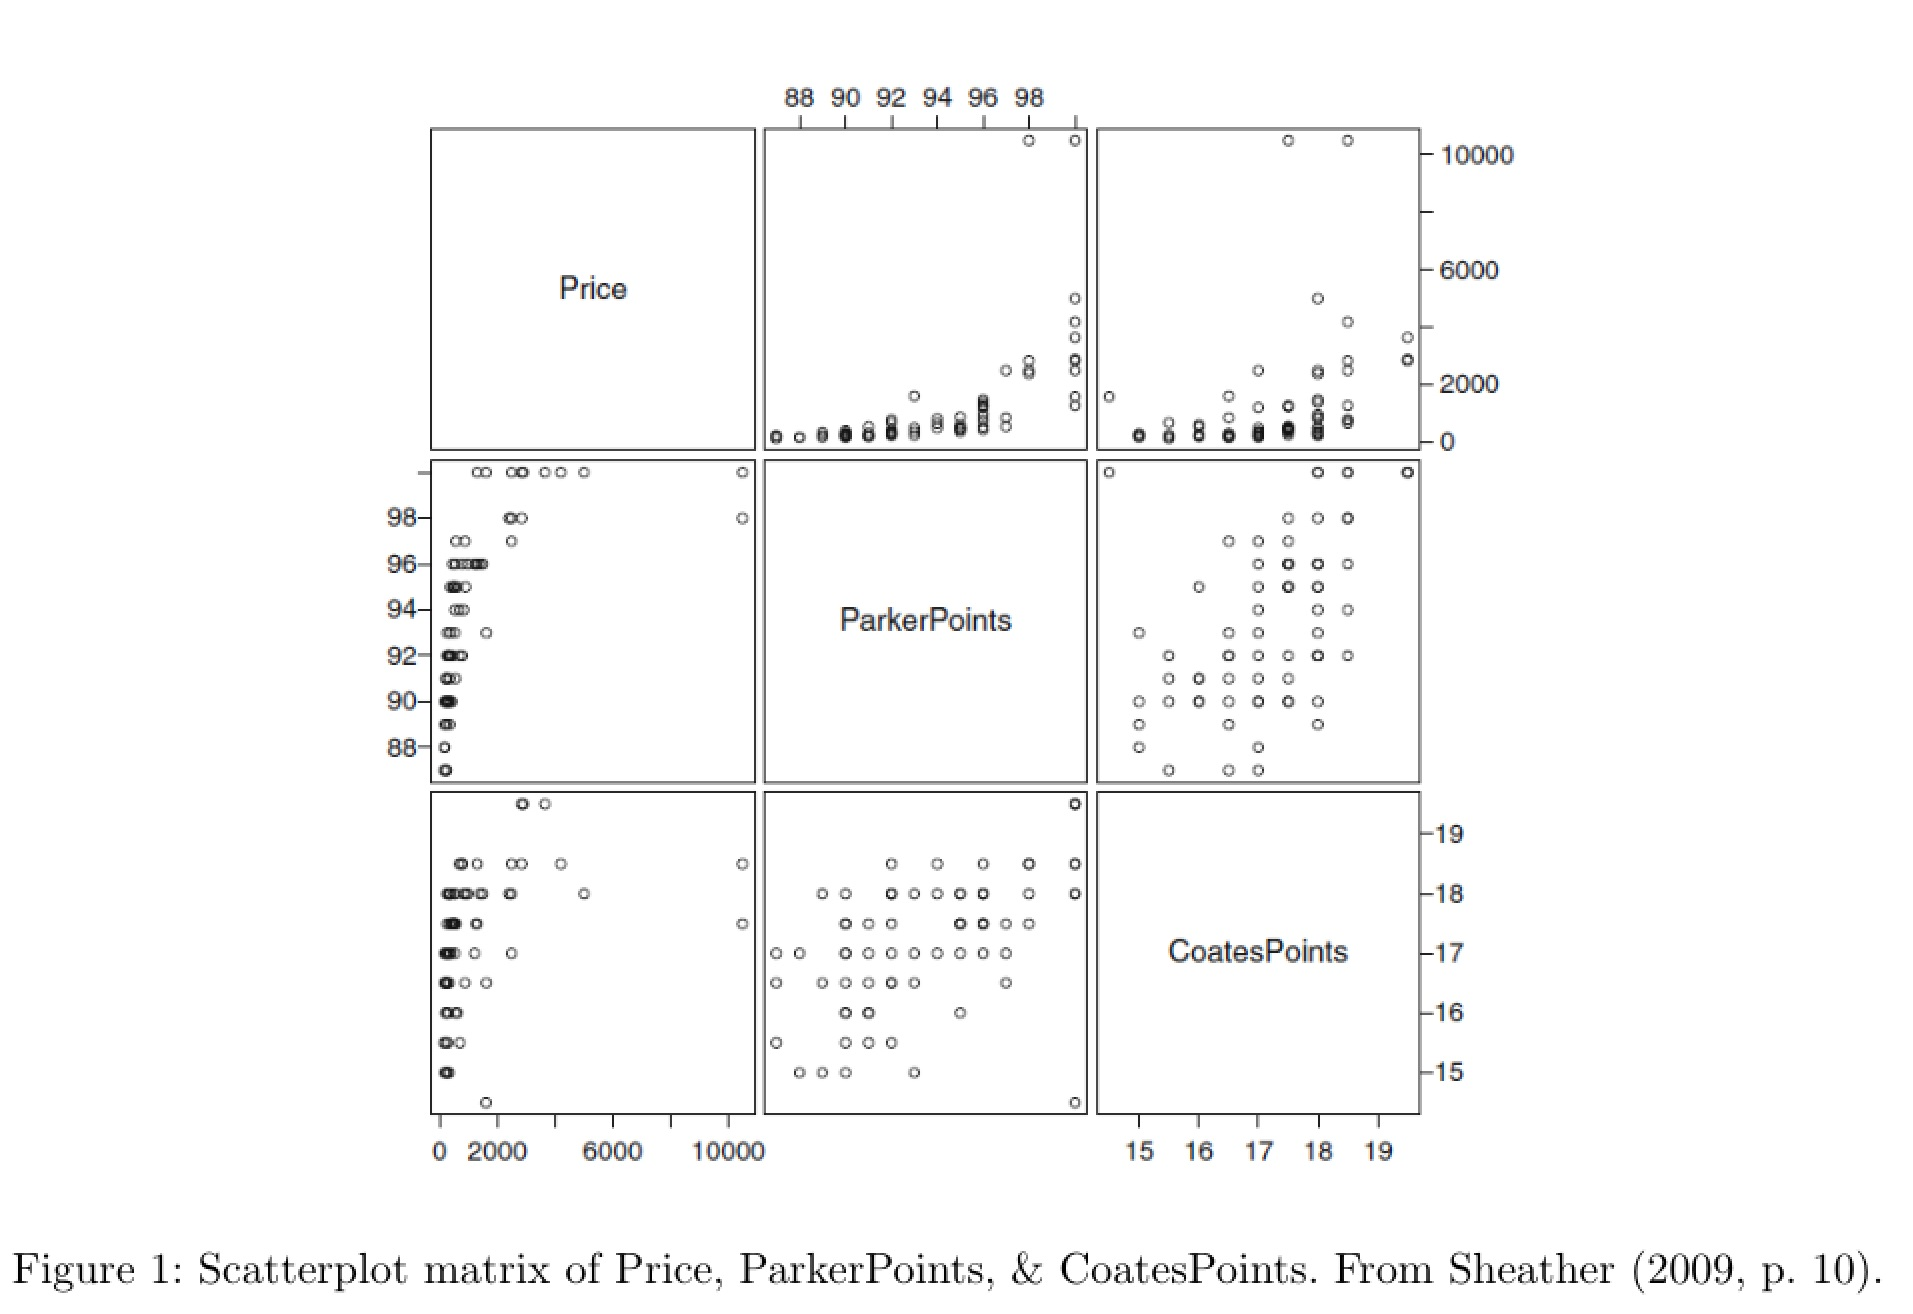
\includegraphics[width=15cm]{Fig01.jpg}
    \label{fig:galaxy}
\end{figure}
We can find out the relationship between Parker and Coates from the slope of the scatterplots in Figure.1.
\begin{figure}[h]
    \centering
    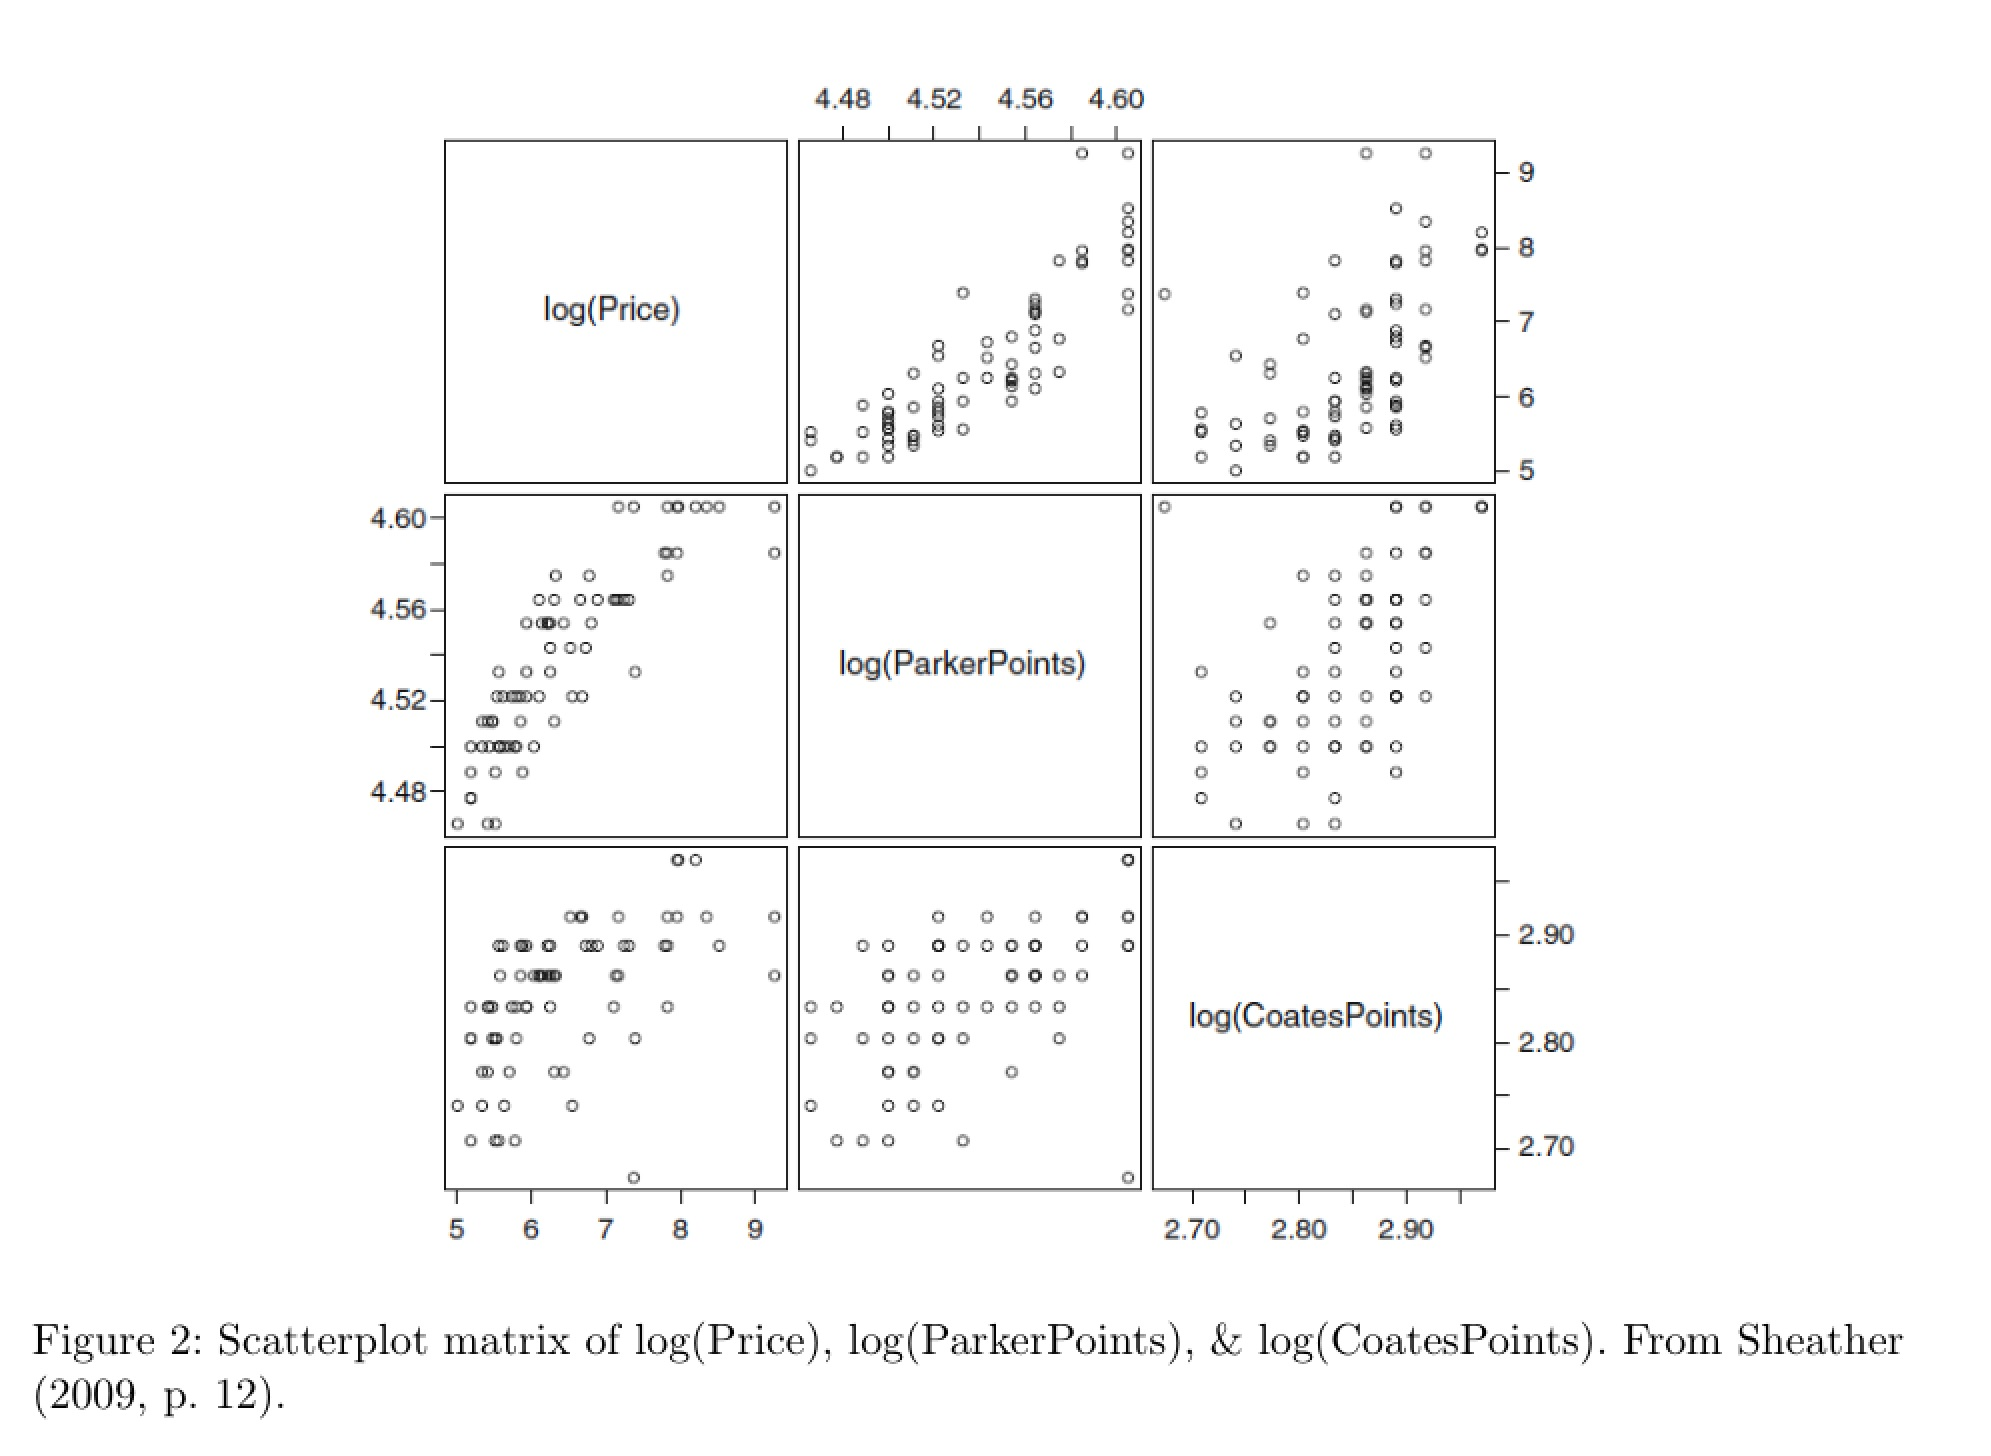
\includegraphics[width=15cm]{Fig02.jpg}
    \label{fig:galaxy}
\end{figure}
However, we find that the relationship between price and the rating is vague in this scatterplot matrix. To find the relationship between the two people's rating systems and the price, we plot the scatterplot matrix(Figure.2) of log(Price), log(ParkerPoints), and log(CoatesPoints).\\\\
\begin{figure}[h]
    \centering
    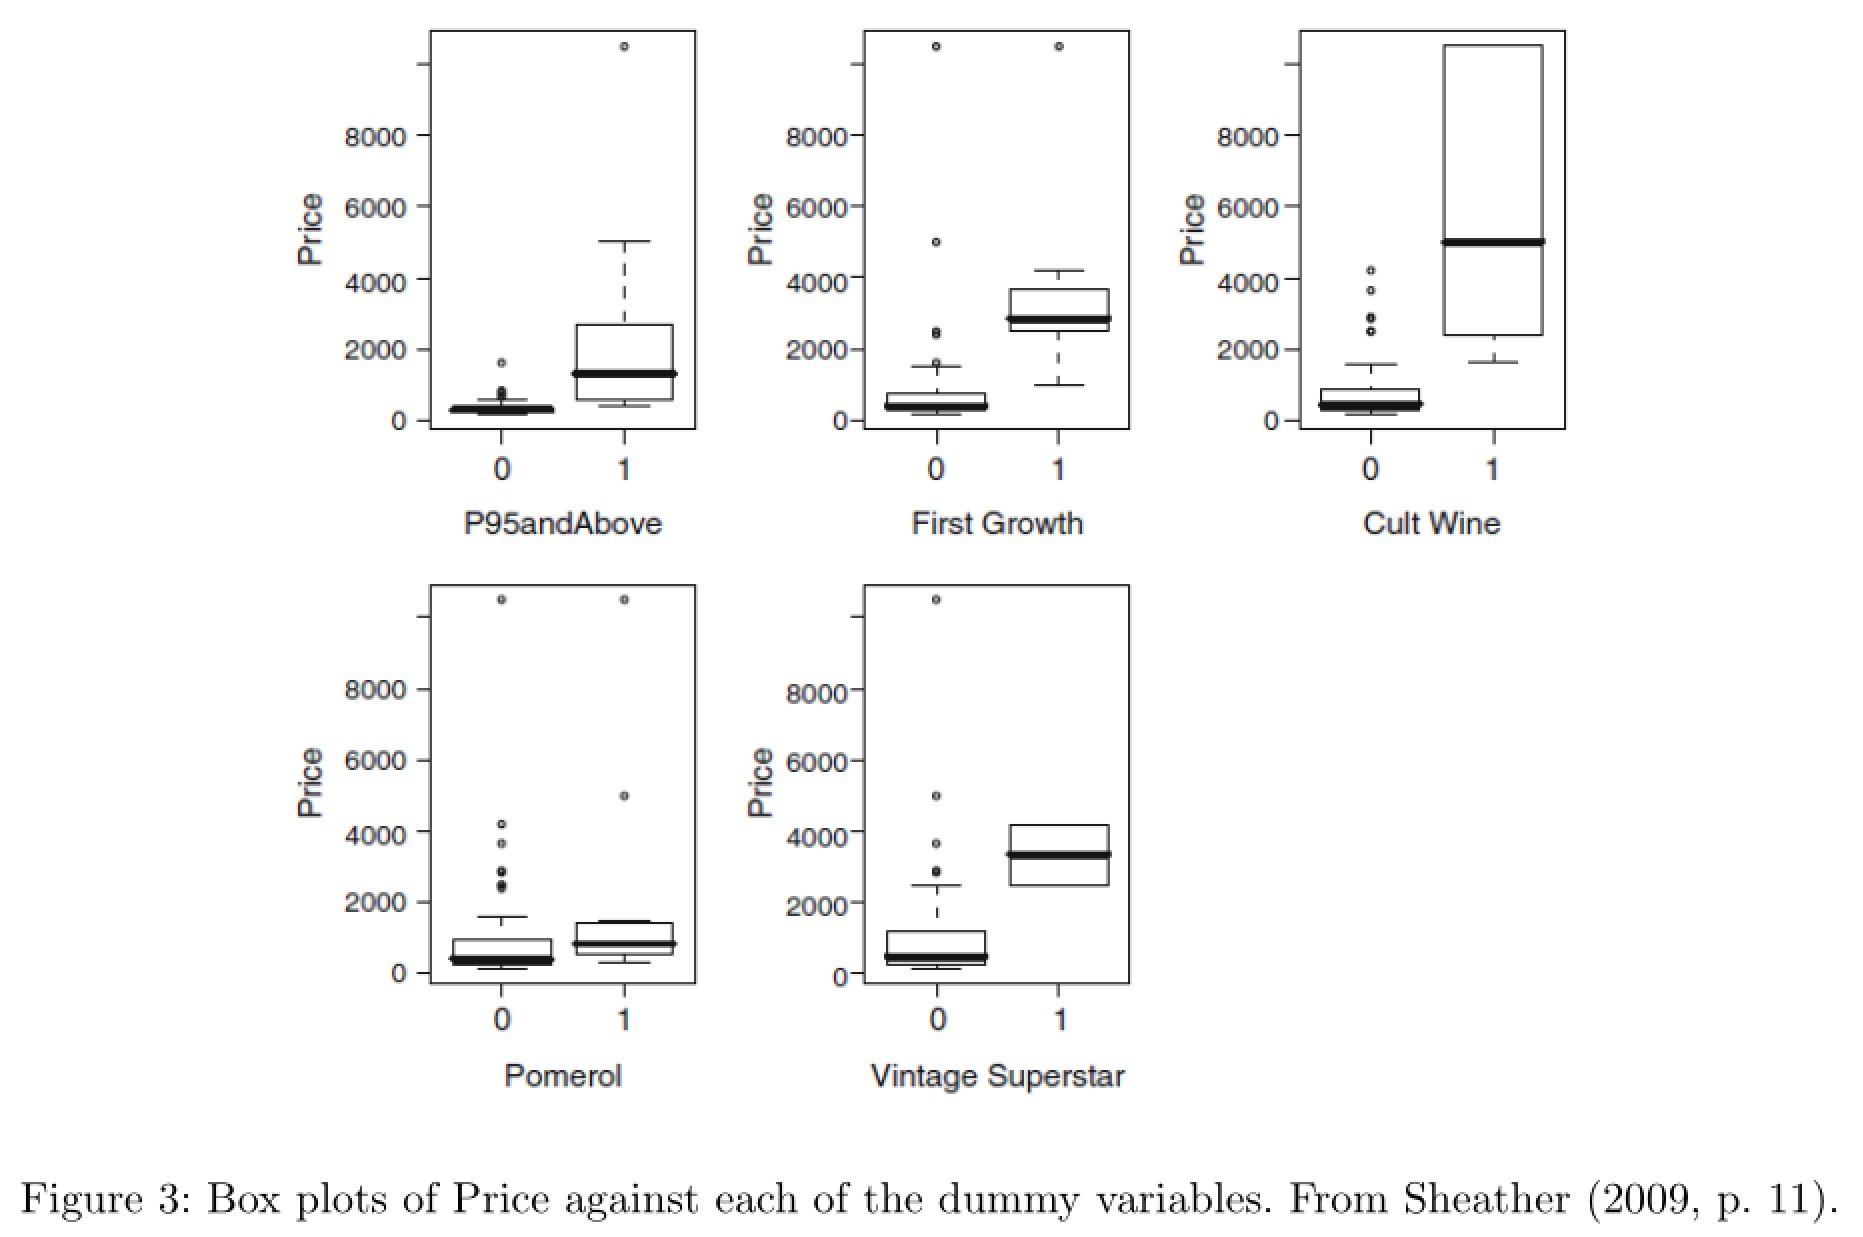
\includegraphics[width=15cm]{Fig03.jpg}
    \label{fig:galaxy}
\end{figure}
Furthermore, to solve the second question, we obtained the box plots(Figure.3) between price and other dummy variables interpreted above. The relationship between these variables are clear in the plots.



\end{document}
